\chapter{Arquitectura software}
\label{cap:capitulo5}

\begin{flushright}
\begin{minipage}[]{10cm}
\emph{Somos lo que hacemos repetidamente, por lo que la excelencia no es un acto, sino un hábito}\\
\end{minipage}\\

Charles Duhigg, \textit{El poder de los hábitos}\\
\end{flushright}

\vspace{1cm}


En este capítulo se describe la topología del sistema utilizado, tanto a nivel software como a nivel hardware. También se describe la forma en la que los diferentes elementos software se complementan, explicando cómo funcionan juntos y detallando los aspectos más importantes de cada uno de ellos.


\section{Estructura hardware}
\label{sec:estructura_hardware}


Para este proyecto se ha usado la Raspberry Pi 4B, debido a su bajo coste y su capacidad de potencia y rapidez con respecto al modelo anterior. El sistema operativo utilizado ha sido Raspberry Pi OS en su versión de 64 bits. Para la conexión de los diferentes sensores y actuadores se han utilizado los puertos \hyperlink{GPIO}{GPIO} ya presentados en la sección \ref{subsec:plataforma_hardware}. En la Figura \ref{fig:circuito} se pueden apreciar las diferentes conexiones de los sensores y actuadores a la Raspberry. A continuación se explicarán los detalles de las conexiones de estos componentes hardware :


\begin{itemize}
 \item \textit{Magnetómetro (Figura \ref{fig:mpu9250}).} Este sensor necesita dos pines SDA y SCL, ya que funciona por conexión I2C, por lo que siguiendo el esquema de la Figura \ref{fig:circuito}, se ha conectado a los pines 3 y 5 respectivamente. También se ha conectado al pin 39(GND) para la toma de tierra y al pin 4 para tener la alimentación de  5V. 
 \item \textit{Micrófono micro USB (Figura \ref{fig:microfono-usb}).} Este sensor se ha conectado en el puerto USB que ofrece la Raspberry de entre los 4 que hay.
 \item \textit{Controlador driver L298N (Figura \ref{fig:l298n}).} Este módulo hardware tiene conectados a la Raspberry los terminales ENA, ENB, IN1, IN2, IN3, IN4 y ENB a los pines 32, 36, 35, 38, 37 y 12 respectivamente. También tiene conectados los terminales GND y VCC a los dos pines de la batería recargable y el mismo terminal GND al pin 34 (GND). Ambos pines de cada motor deben ir conectados a los pines de salida del controlador, OUT1 Y OUT2 para un motor y OUT3 y OUT4 para el otro.
 \item \textit{Powerbank (Figura \ref{fig:Powerbank}).} Esta fuente de alimentación irá conectada al puerto USB-C para proporcionar a la Raspberry los 5V y 3A necesarios.
  \item \textit{HC-SR04 (Figura \ref{fig:hcsr04}).} Esta sensor consta de 4 pines: VCC, GND, TRIG y ECHO. Los 3 primeros irán conectados a los pines 2, 30 y 16 respectivamente. El pin ECHO devuelve 5V y esto podría dañar la Raspberry Pi, ya que sus pines \hyperlink{GPIO}{GPIO} manejan voltajes de 3.3V, por lo que habría que usar un divisor de voltaje con dos resistencias de 1000 $\Omega$ y 2000 $\Omega$ que reducen la señal de 5V a 3.3V y se conectará al pin 18 y al GND a partir de ambas resistencias.
\end{itemize}\


\begin{figure}[H]
  \centering
  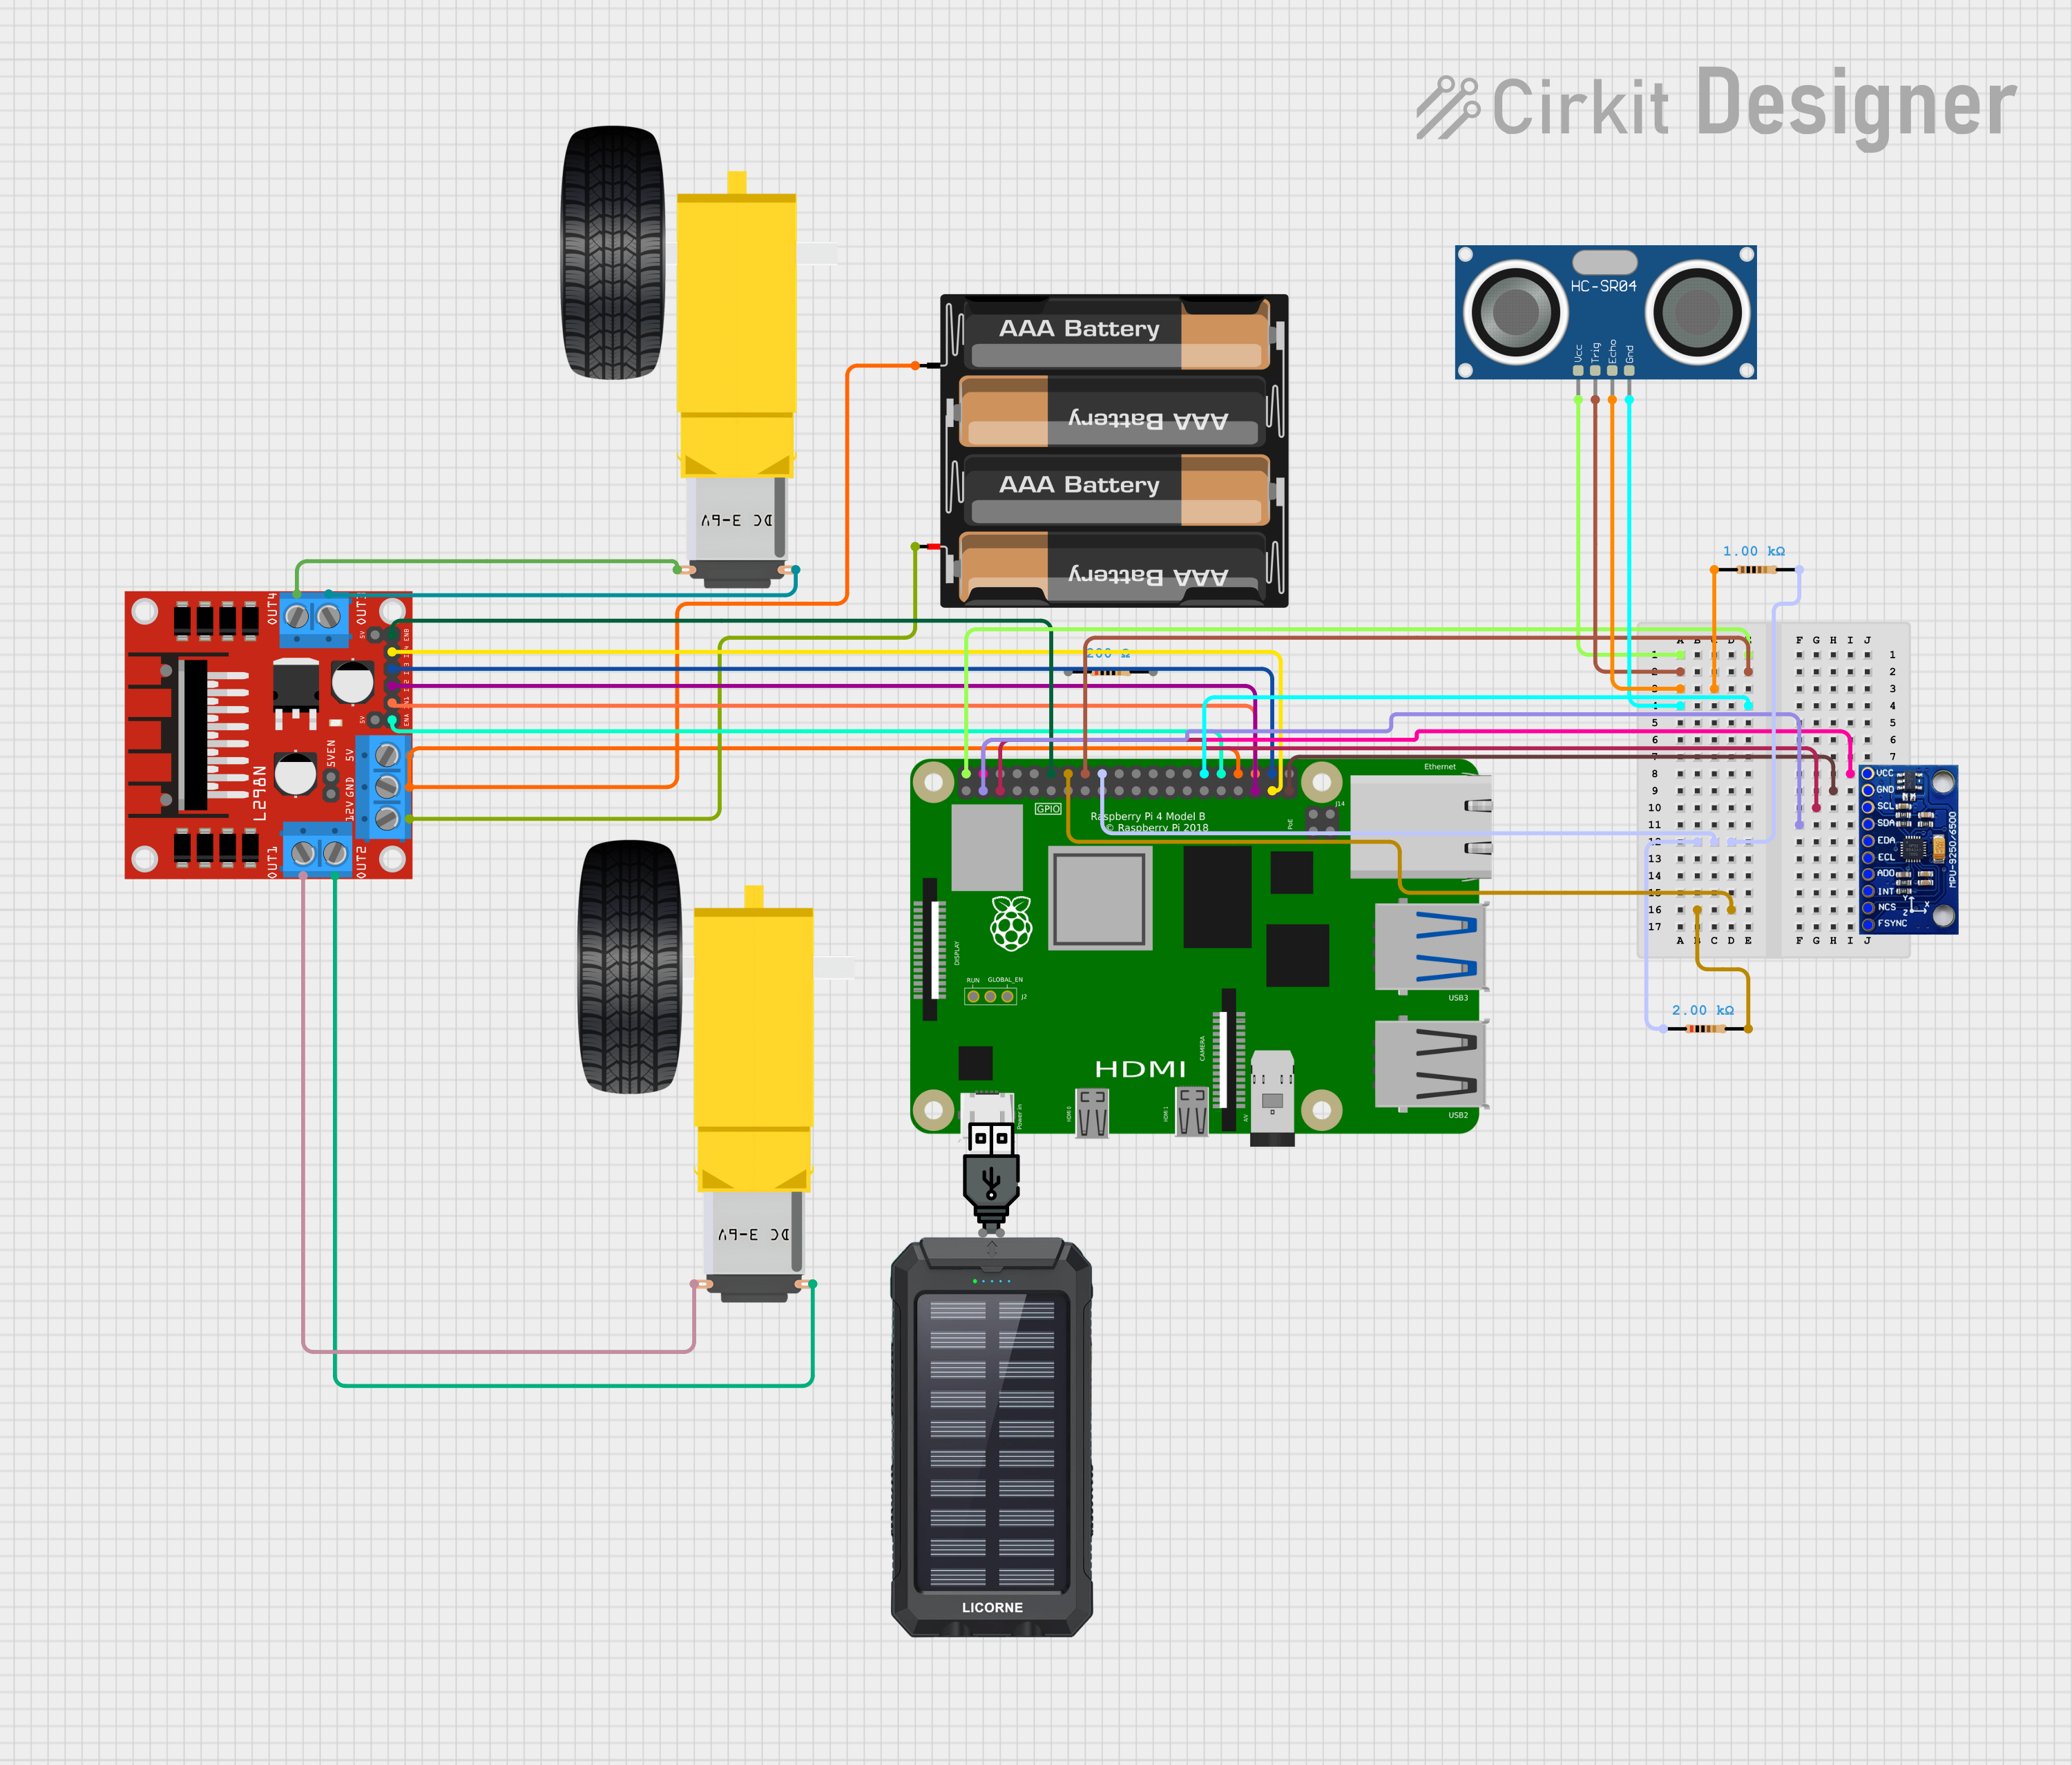
\includegraphics[scale=0.5]{figs/final_circuito} % Escala la imagen al 150% de su tamaño original
  \caption{Esquema de conexiones.}
  \label{fig:circuito}
\end{figure}

\section{Desarrollo software}
\label{sec:desarrollo_software}

Después de diseñar la plataforma hardware, el siguiente paso será darle soporte software, por lo que será necesario calcular el ángulo de orientación del robot, la localización en el mapa, proporcionar un algoritmo que calcule la ruta óptima, y que funcione la red neuronal con distintos comandos por voz, entre otras cosas.


\subsection{Orientación del robot}
\label{subsec:orientacion_robot}

Para poder realizar giros más precisos y tener una trayectoria controlada del robot, es necesario calcular el ángulo de orientación de este dispositivo MPU9250, que como ya se mencionó anteriormente, cuenta con un magnetómetro de 3 ejes, por lo que, utilizando estas lecturas con otras técnicas de calibración, se podrá estimar con alta precisión en que dirección va. Para ello, habrá que actualizar la lista de paquetes, instalar el administrador de paquetes de Python \verb|python3-pip|  e instalar la biblioteca \verb|smbus2| necesaria para I2C, y también la biblioteca \verb|mpu9250-jmdev| específicamente para el MPU9250.



Por otra parte, es muy importante activar el protocolo de I2C para que se pueda comunicar con la Raspberry y le pueda transmitir los datos adquiridos. Esto se activa en: Preferences \texttt{->} Raspberry Pi Configuration \texttt{->} Interfaces \texttt{->} I2C. Si estaba desactivada, es necesario reiniciar la Raspberry. Una vez hecho esto, para ver si lo ha reconocido bien el sensor, habría que ejecutar el comando \textit{i2cdetect -y 1}, el cual dará una tabla que muestra las direcciones I2C de los dispositivos detectados, y habrá que comprobar que detectó un dispositivo. Como se puede apreciar en la Figura \ref{fig:bus}, lo detectó en la dirección 0x68.


\begin{figure}[H]
  \centering
  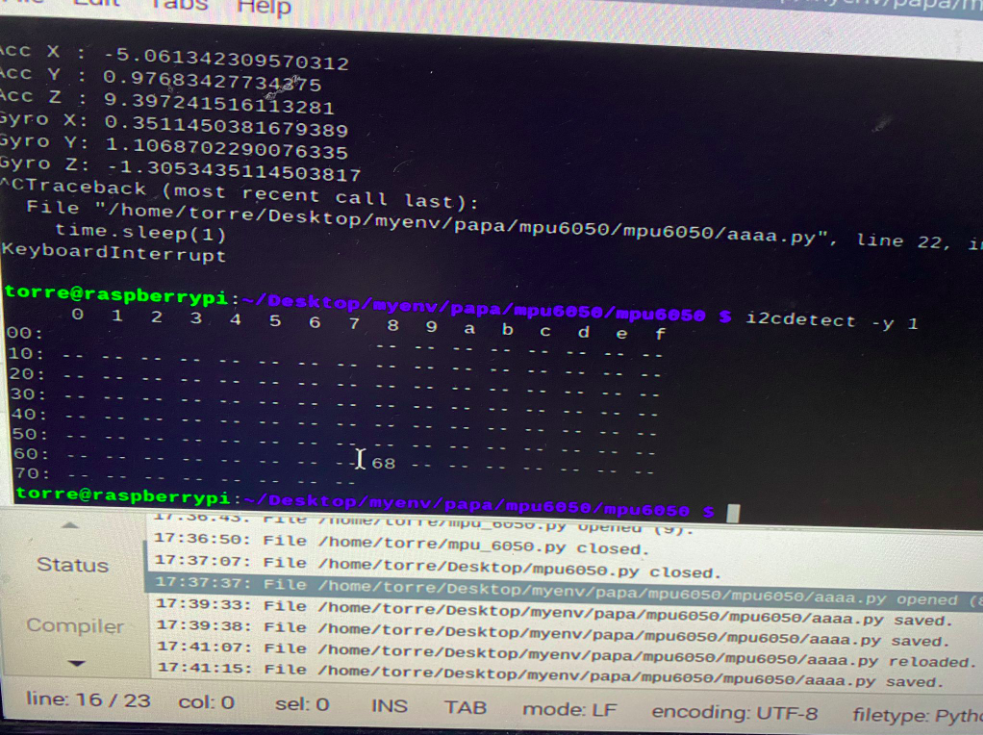
\includegraphics[scale=0.3]{figs/bus} % Escala la imagen al 150% de su tamaño original
  \caption{ Direcciones I2C de los dispositivos detectados.}
  \label{fig:bus}
\end{figure}

El siguiente paso sería obtener las lecturas del magnetómetro. Para ello, habrá que hacer uso de la clase \ref{cod:codejemplo} proporcionada por la biblioteca \texttt{mpu9250\_jmdev}. En primer lugar, se crea una instancia de esta clase con el constructor, con una serie de parámetros que definen la configuración del sensor, que son los siguientes:

\begin{itemize}
 \item \textit{Address\_ak:} Esta es la dirección la cual especifica dónde está conectado el magnetómetro en el bus I2C cuyo valor por defecto es \texttt{AK8963\_ADDRESS}.
 \item \textit{Address\_mpu\_master:} Esta es la dirección I2C del MPU9250 cuyo valor por defecto es \texttt{MPU9050\_ADDRESS\_68}.
 \item \textit{Address\_mpu\_slave:} Esta es la dirección I2C del MPU9250 esclavo si existe, es decir, si se usa un segundo dispositivo cuyo valor por defecto es \textit{None}.
 \item \textit{Bus:} Este es el número del bus I2C que por defecto es 1.
 \item \textit{Gfs:} Este es el rango de sensibilidad del giroscopio que por defecto es \texttt{GFS\_2000 ($\pm 2000^\circ$/seg)}.
 \item \textit{Afs:} Este es el rango de sensibilidad del acelerómetro que por defecto es \texttt{AFS\_16G ($\pm 16G$)}.
 \item \textit{Mfs:} Este es el rango de sensibilidad del magnetómetro que por defecto es \texttt{AK8963\_BIT\_16 (16 bits)}.
 \item \textit{Mode:} Este es el modo de operación del magnetómetro el cual establece el modo de funcionamiento y la frecuencia de muestreo cuyo valor por defecto es \texttt{AK8963\_MODE\_C100HZ}.
\end{itemize}


Luego se configura el sensor para inicializarlo con los parámetros dados mediante el método \verb|configure (self, retry=3)|. El parámetro \textit{retry} es el número de intentos para configurar el sensor que por defecto vale 3 por si ocurre algún error en la configuración, pues se intenta de nuevo las veces que el parámetro retry diga. Dentro de este método, se llama a \verb|configureMPU6500 (gfs, afs)| para configurar el giroscopio y acelerómetro con las escalas determinadas y también se llama a \verb|configureAK8963 (mfs, afs)| para configurar el magnetómetro con el modo y la resolución especificadas y si se agotan los intentos dando error en todos se lanza una excepción.\\


A continuación se capturan los datos del magnetómetro con la función \verb|readMagnetometerMaster (self)| para obtener los 3 componentes del campo magnético medidos en cada uno de los ejes. Primero verifica si hay algún MPU9250 esclavo conectado con el método \verb|hasSlave ()| y si lo hay, lee los datos desde el esclavo con la función \verb|readMaster (EXT_SENS_DATA_14, 7)|, el primer parámetro se corresponde con una dirección específica de un registro en el MPU9250 y el segundo es la cantidad de bytes que se quieren leer.\\

Si no hay ningún esclavo conectado, lee los datos directamente del magnetómetro con la función \verb|readAK (AK8963_MAGNET_OUT, 7))| siendo similar a la anterior. Finalmente, los datos leídos se convierten a unidades compatibles con el método \verb|convertMagnetometer (data)| y si ocurre algún error al leerlos devuelve un valor de error definido por la función \verb|getDataError ()|.\\

Para esta aplicación, solamente se hará uso de las componentes x e y, ya que el objetivo es determinar la dirección del norte magnético en el plano horizontal. La componente z no se utiliza ya que no aporta información relevante, ya que funciona igual que una brújula y ésta misma mide la dirección en el plano horizontal con el ángulo calculado en el plano XY.


\begin{code}[H]
\begin{lstlisting}[language=Python]
class MPU9250:
    def __init__(self, 
        address_ak=AK8963_ADDRESS, 
        address_mpu_master=MPU9050_ADDRESS_68, 
        address_mpu_slave=None, 
        bus=1, 
        gfs=GFS_2000, 
        afs=AFS_16G, 
        mfs=AK8963_BIT_16, 
        mode=AK8963_MODE_C100HZ
    )
       
    def configure(self, retry=3):
        try:
            self.configureMPU6500(self.gfs, self.afs)
            self.configureAK8963(self.mfs, self.mode)
        except OSError as err:
            if(retry > 1):
                self.configure(retry - 1)
            else:
                raise err
     
    def readMagnetometerMaster(self):
        try:
            data = None
            if self.hasSlave():
                data = self.readMaster(EXT_SENS_DATA_14, 7)          
            else:   
                data = self.readAK(AK8963_MAGNET_OUT, 7)
            return self.convertMagnetometer(data)
        except OSError:
            return self.getDataError()           
\end{lstlisting}
\caption[Clase MPU9250]{Clase MPU9250}
\label{cod:codejemplo}
\end{code}


Finalmente, para calcular el ángulo de orientación, habrá que hacer uso de la función \verb|math.atan2 (y,x)| para calcular el ángulo entre el vector formado por los parámetros XY y el eje positivo X, siendo x e y las lecturas magnéticas medidas por el magnetómetro. Este ángulo está en radianes por lo que habría que pasarlo a grados multiplicando por 180 y dividiendo entre \(\pi\).\\

La función \verb|math.atan2 (y,x)| puede devolver un valor negativo en ciertos casos, y lo ideal es que se mantenga en el rango de 0º y 360º mediante esta condición \ref{cod:codejemplo3}.


\begin{code}[H]
\begin{lstlisting}[language=Python]
if heading_angle_in_degrees < 0:
    heading_angle_in_degrees += 360
\end{lstlisting}
\caption[Mantener el ángulo en el rango correcto]{Mantener el ángulo en el rango correcto}
\label{cod:codejemplo3}
\end{code}


Es importante tener en cuenta también el concepto de declinación magnética, que es el ángulo que existe entre el norte verdadero(Polo Norte geográfico) y el norte magnético que es la dirección hacia el Polo Norte magnético que cambia con el tiempo. Una brújula normal apunta al norte magnético y no al norte verdadero. En este proyecto no se tendrá en cuenta esta desviación, que es diferente dependiendo del lugar, ya que al ser en interiores no varía casi nada este factor pero si fuese en exteriores sí que habría que tenerlo en cuenta. Para saber la declinación magnética de un lugar específico de la Tierra se puede hacer uso de esta página web\footnote{\url{https://www.magnetic-declination.com/}}.\\


Una vez obtenido el ángulo de orientación, se comprueba que las medidas no son exactas y varían mucho, por lo que es necesario calibrar el dispositivo como se muestra en la Sección \ref{sec:cal_mag}.



\subsection{Diseño del mapa}
\label{subsec:diseño_mapa}

Dentro de la navegación global, el robot parte de un mapa conocido gestionado de la siguiente forma. Primero, se hace uso de la herramienta \hyperlink{GIMP}{GIMP}, como ya se mencionó en la Sección \ref{subsec:gimp} para la edición de imágenes, en la que se tendrá un fondo en blanco y se pintarán de color negro aquellos píxeles que representen obstáculos para el robot y también los \hyperlink{APs}{APs} como se puede apreciar en la Figura \ref{fig:mapa_apes}, ya que se consideran obstáculos por donde no podrá pasar el robot\footnote{En este caso se pintaron de azul para poder distinguirse de un obstáculo normal aunque en el mapa final irán pintados en color negro}.

\begin{figure}[H]
  \centering
  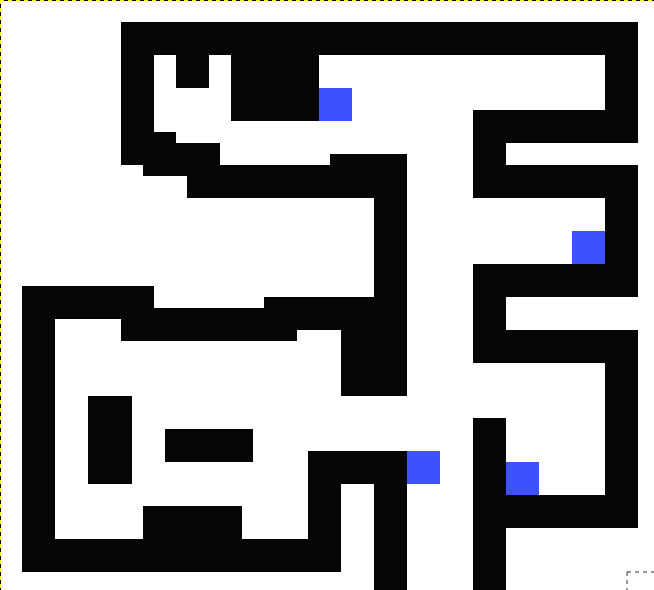
\includegraphics[scale=0.3]{figs/mapa_apes} % Escala la imagen al 150% de su tamaño original
  \caption{ Mapa de ejemplo en GIMP con los APs establecidos.}
  \label{fig:mapa_apes}
\end{figure}

Los píxeles de alrededor de estos obstáculos también se pintarán de color negro para tener un margen de seguridad en los cálculos de movimiento junto con los \hyperlink{APs}{APs} como se puede apreciar en este mapa de ejemplo final (Figura \ref{fig:mapa_apes}):


\begin{figure}[H]
  \centering
  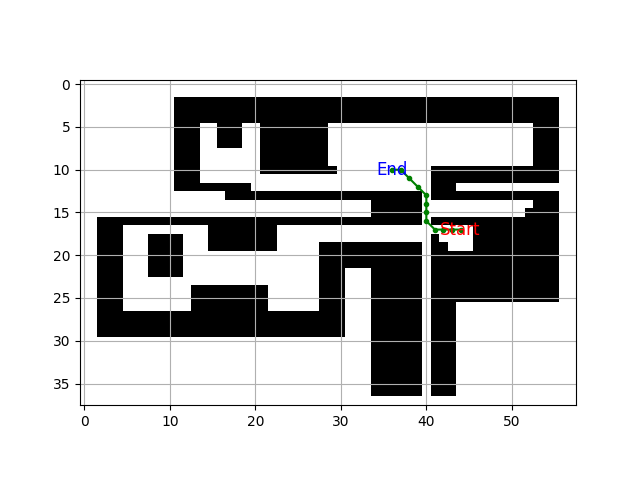
\includegraphics[scale=0.8]{figs/astar} % Escala la imagen al 150% de su tamaño original
  \caption{ Ejemplo del mapa final con los obstáculos ampliados.}
  \label{fig:astar}
\end{figure}

Los colores de cada píxel del mapa tienen importancia y se ha diseñado así ya que el algoritmo de navegación trabaja con una matriz de 0 y 1 por la cual navegará el robot por los valores de la matriz que tienen un 1 que representa el color blanco. Una vez exportada la imagen en formato png, se hará uso de esta Función \ref{cod:codejemplo4}, la cual recorre los píxeles de la imagen viendo los valores de cada uno y escribe un 0 o 1 dependiendo del color del píxel, aceptando como parámetros la imagen y un archivo vacío en formato txt en la que se escribirá la matriz.

\begin{code}[H]
\begin{lstlisting}[language=Python]
def image_to_binary_text(image_path, output_file):
    # Abrir la imagen en blanco y negro
    img = Image.open(image_path).convert('1') 

    width, height = img.size
   
    with open(output_file, 'w') as f:
        # Iterar sobre cada pixel de la imagen
        for y in range(height):
            for x in range(width):
                pixel = img.getpixel((x, y))

                bit_value = '0' if pixel == 0 else '1'

                f.write(bit_value)

            f.write('\n') 
\end{lstlisting}
\caption[Función para convertir una imagen en representación binaria ]{Función para convertir una imagen en representación binaria}
\label{cod:codejemplo4}
\end{code}

Finalmente el archivo de salida con la representación binaria de la matriz (Figura \ref{fig:bin}) es la que se le pasará al algoritmo de navegación A* para poder navegar por ella. 

\begin{figure}[H]
  \centering
  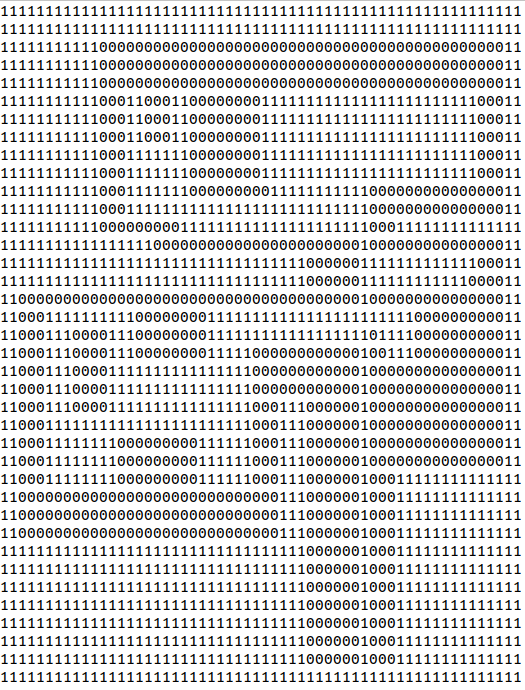
\includegraphics[scale=0.5]{figs/bin} % Escala la imagen al 150% de su tamaño original
  \caption{ Ejemplo de la representación binaria del mapa.}
  \label{fig:bin}
\end{figure}


\subsection{Interfaz de usuario}
\label{subsec:interfaz_usuario}

Una de las mejores formas de interactuar con el robot es mediante comandos de voz ya que es muy natural e intuitivo para los usuarios. El primer paso sería tener un dataset de audios de prueba en español con los comandos de voz que reconocerá el robot. Estos audios deben ir en formato WAV, ya que a diferencia del formato MP3, el formato WAV es un formato de audio sin pérdida, por lo que no hay compresión con pérdida de información auditiva y cada vez que un archivo MP3 se comprime, se pierde cierta información para reducir el tamaño del archivo y podría afectar la calidad del sonido y al rendimiento de la red neuronal si la calidad del audio es crucial y en este caso sí lo es. Al no haber pérdidas en el formato WAV, aumentan los bytes de cada audio por lo que para que se puedan clasificar correctamente, tras diferentes pruebas realizadas cada audio no podrá superar los 200 bytes.\\

Las clases deberían estar equilibradas para facilitar la tarea de entrenamiento; es decir, debería de haber el mismo número de audios para cada clase. Cada audio tiene asignado un número que representa la clase a la que pertenece, como por ejemplo \texttt{ej1-01-.wav}. Las diferentes clases representan los diferentes comandos que hay.\\


 El siguiente paso sería cargar cada uno de los audios y extraer las características de cada uno de ellos para calcular la transformada de Fourier del espectrograma del audio (\hyperlink{STFT}{STFT}), los coeficientes cepstrales de frecuencias mel (\hyperlink{MFCC}{MFCC}) y los espectrogramas mel, ya que son propiedades que usará el modelo para clasificar cada archivo de audio. Para calcular estas características, primero se calcula la forma de onda para diferentes audios (Figura \ref{fig:onda}), y se puede observar que hay una diferencia visible, pero no la suficiente para clasificarla.
 
 \begin{figure}[H]
  \centering
  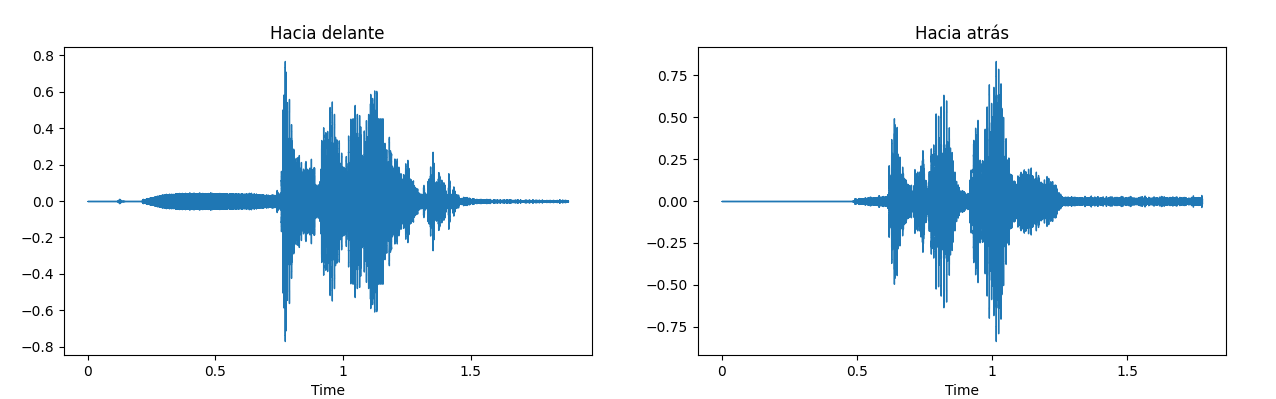
\includegraphics[scale=0.3]{figs/forma_onda} % Escala la imagen al 150% de su tamaño original
  \caption{ Forma de onda de diferentes audios.}
  \label{fig:onda}
\end{figure}



Para calcularla basta con abrir el archivo y leer los datos de audio en formato \texttt{float32} que es un formato estándar para procesar señales de audio. De esta manera, convierte la señal en un array en la que cada elemento representa la amplitud del audio guardado en \texttt{waveform}. También se calcula la frecuencia de muestreo que será necesaria para después.

\begin{verbatim}
with soundfile.SoundFile(file) as audio:
        waveform = audio.read(dtype="float32")
        sample_rate = audio.samplerate
\end{verbatim}

Para poder calcular la \hyperlink{STFT}{STFT} (Figura \ref{fig:stft}) se hace uso de la función \verb|feature_chromagram (waveform, sample_rate)|, la cual toma la forma de onda y la frecuencia de muestreo y calcula la \hyperlink{STFT}{STFT} del audio que descompone la señal en sus componentes de frecuencia a lo largo del tiempo y toma su valor absoluto, teniendo así una matriz en la cual las columnas representan los frames de tiempo y las filas representan las frecuencias. Luego lo convierte en un cronograma (Figura \ref{fig:cronograma}) que mide la energía de cada una de las notas musicales presentes en el frame, siendo una matriz cambiando las filas que son las notas musicales con las columnas (frames) y finalmente calcula la media de cada columna teniendo así un vector de 12 componentes en la que cada elemento representa la energía media de una nota en todo el audio.


\begin{code}[H]
\begin{lstlisting}[language=Python]
def feature_chromagram(waveform, sample_rate):
    stft_spectrogram=np.abs(librosa.stft(waveform))
    chromagram=np.mean(librosa.feature.chroma_stft(S=stft_spectrogram, sr=sample_rate).T,axis=0)
    return chromagram
\end{lstlisting}
\caption[Función para calcular la STFT de un audio]{Función para calcular la STFT de un audio}
\label{cod:codejemplo6}
\end{code}

\begin{figure}[H]
  \centering
  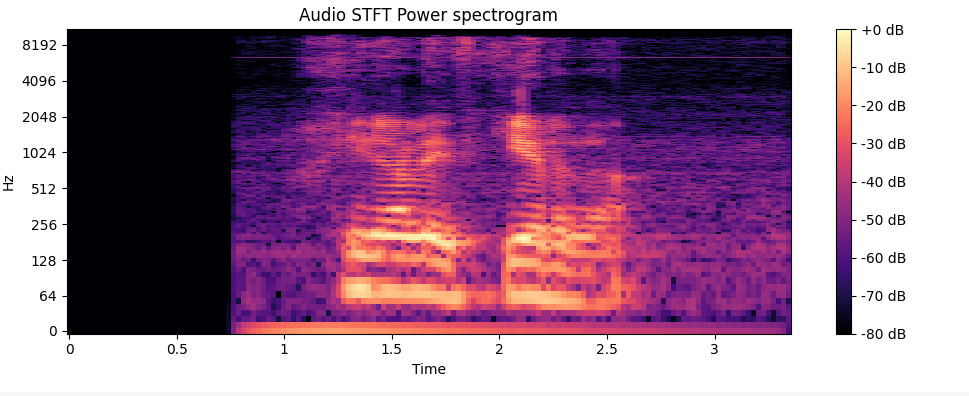
\includegraphics[scale=0.4]{figs/stft_spectogram} % Escala la imagen al 150% de su tamaño original
  \caption{ Representación de la transformada de Fourier de corta duración de un audio.}
  \label{fig:stft}
\end{figure}

\begin{figure}[H]
  \centering
  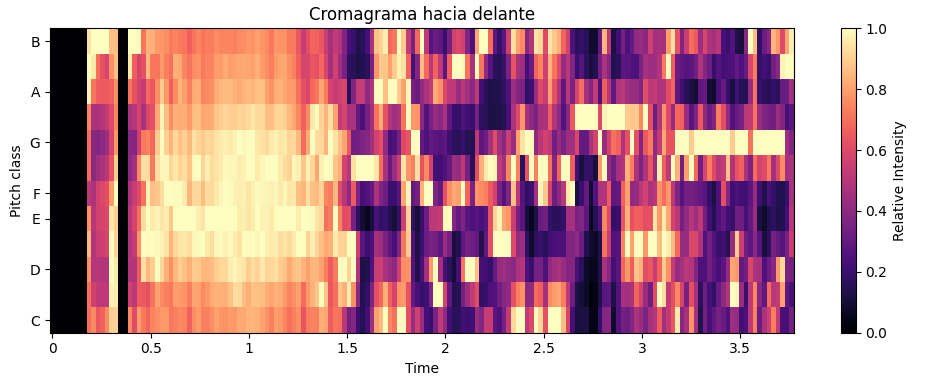
\includegraphics[scale=0.4]{figs/cromagrama} % Escala la imagen al 150% de su tamaño original
  \caption{ Representación del cronograma de un audio.}
  \label{fig:cronograma}
\end{figure}


Con la forma de onda y la frecuencia de muestreo, también se puede calcular los coeficientes \hyperlink{MFCC}{MFCC} (Figura \ref{fig:mfcc}) que nos dan una idea del tono cambiante de una señal de audio. Con la función \verb|feature_mfcc (waveform, sample_rate)|, se calculan los \hyperlink{MFCC}{MFCC} de una señal y en este caso como indica el parámetro \texttt{n\_mfcc} se calculan 40 coeficientes para tener más detalles del contenido espectral, ya que para esta tarea 40 coeficientes proporcionan la mejor precisión y un cálculo rápido. El atributo ``\texttt{.T}" transpone la matriz intercambiando así los coeficientes con los fotogramas de tiempo y luego se calcula la media de cada columna generando así un vector de tamaño 40.


\begin{code}[H]
\begin{lstlisting}[language=Python]
def feature_mfcc(waveform, sample_rate):
    mfc_coefficients=np.mean(librosa.feature.mfcc(y=waveform, sr=sample_rate, n_mfcc=40).T, axis=0)
    return mfc_coefficients
\end{lstlisting}
\caption[Función para calcular los espectrogramas mel de un audio]{Función para calcular los espectrogramas mel de un audio}
\label{cod:codejemplo5}
\end{code}

\begin{figure}[H]
  \centering
  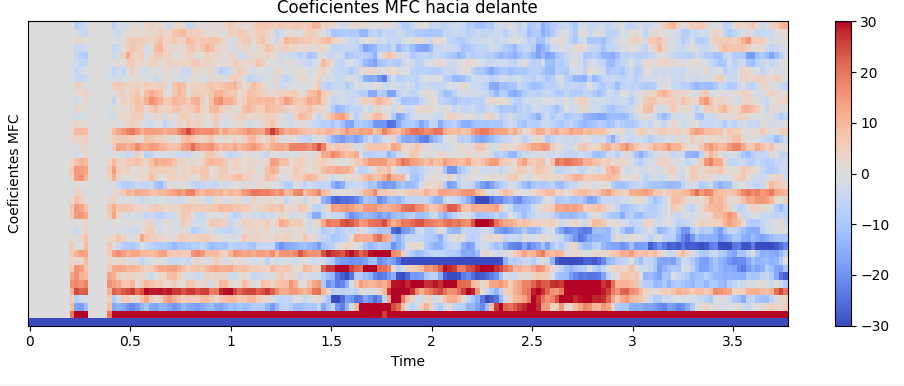
\includegraphics[scale=0.4]{figs/coeficientes_mfc} % Escala la imagen al 150% de su tamaño original
  \caption{ Representación de los coeficientes MFCC de un audio.}
  \label{fig:mfcc}
\end{figure}

Como derivado de los cálculos anteriores se pueden calcular los espectrogramas mel (Figura \ref{fig:mel}) que serán otra buena función para analizar y observar más detalladamente cómo son las transiciones entre los picos de frecuencias mel. Con la función \verb|feature_melspectrogram (waveform, sample_rate)|, se consiguen las características en forma de espectrograma mel el cual se asemeja cómo los humanos perciben las frecuencias. \texttt{N\_mels} se corresponde con el número de bandas en la escala mel con lo que se genera un espectrograma con 128 características y \texttt{f\_max} es la frecuencia máxima y para la mayoría de tareas de clasificación por voz 8kHz es suficiente. El atributo ``\texttt{.T}" transpone la matriz del espectrograma mel intercambiando así las bandas mel(filas) con los fotogramas de tiempo(columnas) y luego se calcula la media de cada columna generando así un vector de tamaño 128 en la que cada valor representa la energía media de una banda mel.



\begin{code}[H]
\begin{lstlisting}[language=Python]
def feature_melspectrogram(waveform, sample_rate):
    melspectrogram=np.mean(librosa.feature.melspectrogram(y=waveform, sr=sample_rate, n_mels=128, fmax=8000).T,axis=0)
    return melspectrogram
\end{lstlisting}
\caption[Función para calcular los espectrogramas mel de un audio]{Función para calcular los espectrogramas mel de un audio}
\label{cod:codejemplo5}
\end{code}

\begin{figure}[H]
  \centering
  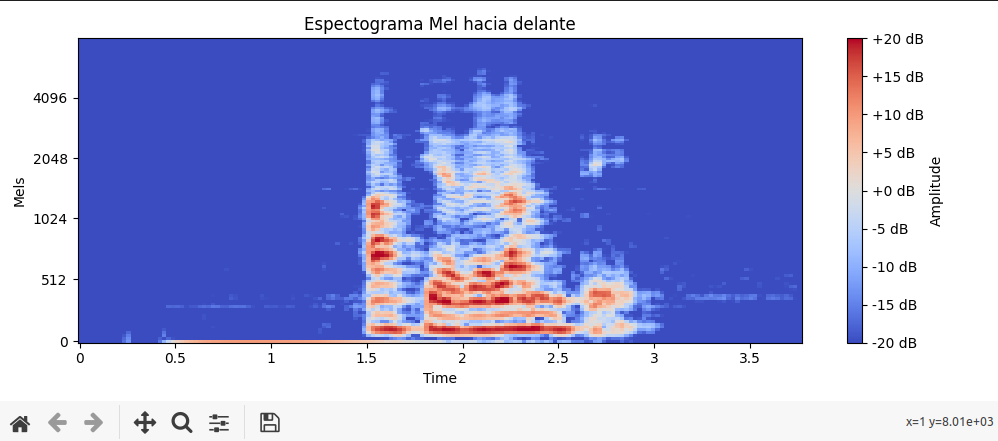
\includegraphics[scale=0.4]{figs/mel_spectrogram} % Escala la imagen al 150% de su tamaño original
  \caption{ Representación de los espectrogramas mel de un audio.}
  \label{fig:mel}
\end{figure}

Ya con todo esto se tendrían 180 características, de las cuales 128 pertenecerían al número de bandas mel que se utilizan para calcular el espectrograma mel, ya que se ha establecido en 128 porque funciona óptimamente,ya que valores más altos pueden proporcionar una representación más detallada pero también pueden requerir más recursos computacionales. Otras 40 saldrían de establecer 40 \hyperlink{MFCC}{MFCC}, aunque al igual que el anterior parámetro no hay un número fijo. Las otras 12 restantes serían las del cromagrama, una para cada una de las 12 clases de tonos.

Una vez calculadas las 180 características para cada uno de los audios se agruparán en una matriz los audios totales que haya en el dataset para poder representarlos correctamente de esta manera:

\begin{verbatim}
feature_matrix = np.hstack((chromagram, melspectrogram, mfc_coefficients))
\end{verbatim}

Como estas características tienen magnitudes diferentes, es necesario escalarlas para normalizar los datos y que las características tengan una escala comparable, mejorando así la estabilidad y el rendimiento del modelo, ya que se obtenía que la desviación de los coeficientes \hyperlink{MFCC}{MFCC} era mayor que la de las demás características. 

Para el escalado se usó la función \verb|StandardScaler ()| de sklearn que resta la media de cada característica y la divide por la desviación estándar de esa característica, produciendo características con media cero y varianza unitaria, por lo que los valores extremos tendrán menos impacto en los pesos aprendidos del modelo y el modelo es menos sensible a los valores atípicos. 

El siguiente paso sería elegir el modelo que se va a usar y como se podrá observar más adelante, se usará el modelo Random Forest para entrenar a la red ya que en el experimento descrito en la Sección \ref{sec:eleccion_modelo}, se observó el rendimiento de cada uno de los modelos y el más fiable era el de RandomForestClassifier, junto con la clasificación por vectores de apoyo \hyperlink{SVC}{SVC} (Support Vector Classification).

El proceso final sería cargar el modelo ya entrenado, ejecutar mediante el módulo \texttt{subprocess} el comando arecord para grabar un audio, obtener las características del audio y pasárselas al modelo para que haga la predicción correcta en la respectiva clase del audio al que pertenece. El comando arecord tiene diferentes parámetros como los siguientes: 

\begin{verbatim}
arecord -t wav -d 2 -r 44000 -c 1 ej20-01-.wav 
\end{verbatim}

El parámetro -t wav especifica el tipo de archivo de audio como WAV, -d 2 establece la duración de la grabación en 2 segundos, -r establece la frecuencia de muestreo en 44,000 Hz, -c 1, especifica que se desea grabar con un solo canal (mono). Esto último es importante ya que en este caso solo se usa un canal para transmitir el sonido y si se graba como -c 2 se estará usando un canal estéreo que usa dos canales por lo que al pasárselo a la red dará problemas.


\subsection{Localización}
\label{subsec:localización}

Al navegar en interiores, la tecnología GPS no es adecuada para esta tarea ya que la señal es débil y puede proporcionar un error muy alto, por lo que se ha usado un sistema de posicionamiento basado en la utilización de balizas WiFi para obtener una estimación de la posición del robot mediante los valores \hyperlink{RSSI}{RSSI} para obtener la distancia y con la posición en la que se ubican en el mapa los \hyperlink{APs}{APs}. Para conectarse a un AP se utilizará esta función \ref{cod:codejemplo6}, en la cual se usa el comando \texttt{subprocess.run} para ejecutar \texttt{nmcli} especificando la red(en este caso WiFi), la acción para conectarse a ella junto con el nombre de la red y la contraseña y con \texttt{check=True} hace que se genere una excepción si falla el comando.\\

\begin{code}[H]
\begin{lstlisting}[language=Python]
def connect_to_wifi(ssid, password):
    try:
        subprocess.run(["nmcli", "d", "wifi", "connect", ssid, "password", password], check=True)
        print(f"Conectado a {ssid}")
    except subprocess.CalledProcessError as e:
        print(f"Error al conectar a {ssid}: {e}")
\end{lstlisting}
\caption[Función para conectarse a una red WiFi]{Función para conectarse a una red WiFi}
\label{cod:codejemplo6}
\end{code}

Una vez se tiene la potencia recibida del AP, para calcular la distancia hay que usar esta ecuación \ref{ec:ec2}:




\begin{myequation}[H]
\begin{equation}
d = 10^{\frac{A - \texttt{\hyperlink{RSSI}{RSSI}}}{10 \cdot n}}
\label{ec:ec2}
\end{equation}
\caption[Ecuación para calcular la distancia a un AP]{Ecuación para calcular la distancia a un AP}
\end{myequation} 
\texttt{Donde:}
\begin{itemize}
    \item $d$: Distancia estimada en metros.
    \item $A$: Valor \hyperlink{RSSI}{RSSI} a 1 metro del AP.
    \item \texttt{\hyperlink{RSSI}{RSSI}}: Potencia recibida.
    \item $n$: Factor de propagación (depende del entorno, generalmente es 2-3 en interiores).
\end{itemize}


Teniendo ya la distancia a cada AP y sabiendo la posición de cada uno de ellos en el mapa, mediante múltiples puntos de referencia se puede usar la trilateración y calcular la posición del robot. Para ello se puede usar este sistema de ecuaciones \ref{ec:ec5}. 




\begin{myequation}[H]
\begin{equation}
\left\{
	\begin{array}{lcc}
		(x - x_1)^2 + (y - y_1)^2 = (d_1)^2\\
		(x - x_2)^2 + (y - y_2)^2 = (d_2)^2\\
		(x - x_3)^2 + (y - y_3)^2 = (d_3)^2 \\
		(x - x_4)^2 + (y - y_4)^2 = (d_4)^2
	\end{array}
\right.
\label{ec:ec5}
\end{equation}
\caption[Sistema de ecuaciones para calcular la posición dada la distancia y la posición de cada AP]{Sistema de ecuaciones para calcular la posición dada la distancia y la posición de cada AP}
\end{myequation}


El siguiente paso sería averiguar cuántos \hyperlink{APs}{APs} son necesarios para estimar la posición y que haya el mínimo de error. Para ello se realizará un experimento \ref{sec:num_aps} en el cual se comprobará esto último y también se hará un estudio sobre el impacto que tiene el espacio que hay entre las cuadrículas del mapa sobre el cálculo de la posición del robot.


\subsection{Navegación}
\label{subsec:navegación}

Un problema a tratar es la navegación, y al tener una batería tan limitada no se puede hacer que se desplace grandes distancias, por lo que se tratará la navegación en interiores. En cuanto a la navegación global, es necesario implementar un algoritmo de navegación óptimo como el de A*. Este algoritmo combina características de los algoritmos de búsqueda de costo uniforme y búsqueda heurística, lo que lo hace eficiente y efectivo en la resolución de problemas de planificación de rutas. 

Dada una lista de datos o valores, este algoritmo buscará iterativamente los datos requeridos o
valor solicitado dentro de la lista, en este caso la matriz de 0 y 1 como se mencionó anteriormente. 

Después de considerar los criterios de compensación de optimalidad, completitud, precisión y el tiempo de ejecución, se ha determinado que el algoritmo de planificación de rutas A*
sería el más adecuado para el entorno simulado que se quiere probar. 


A* es lo que se considera un algoritmo de búsqueda Best-First, lo que significa que se tomará el movimiento de menor costo por iteración. Esto significa que se elige la ruta más cercana y eficiente que sea inmediatamente visible, analizando todos los posibles caminos más cortos. A* siempre encontrará una solución si existe una, lo que lo convierte en un algoritmo de búsqueda óptimo. Este algoritmo pretende minimizar el coste del camino cogido mediante la ecuación:


\begin{myequation}[H]
\begin{equation}
\left\{
	f(n) = g(n) + h(n)
\right.
\label{ec:ec6}
\end{equation}
\caption[Fórmula de la función de costo]{Fórmula de la función de costo}
\end{myequation}


Donde g(n) es el costo de cada movimiento desde el nodo inicial hasta el nodo final, y h(n) es la
heurística en la que se estiman los costos futuros. La heurística es una estimación o evaluación del costo de
movimientos futuros. Al sumar el costo estimado de los movimientos futuros y los pasos ya realizados, se puede estimar el camino de menor costo a recorrer.


El proceso final consistiría entonces en pasarle al algoritmo la imagen binaria del mapa de 0 y 1 y transformarla en una matriz con la cual trabajará el algoritmo, junto con el punto de partida y el objetivo final. Para encontrar el camino se verifica primero si el origen y el destino son válidos y si el punto inicial ya es el destino finaliza. Luego, se define la celda de inicio con los costos y la heurística a 0 dentro de otra matriz de objetos y se agrega a la cola de prioridad junto con sus coordenadas. En el bucle principal se sacará el nodo con menor f(n) de la cola de prioridad y expandiendo así el nodo con menor costo total y marcándola como visitada para no volver a procesarla. Después de esto se seguirán expandiendo los nodos vecinos y actualizando los costos y agregándolos a la cola de prioridad hasta encontrar el destino.

\begin{figure}[H]
  \centering
  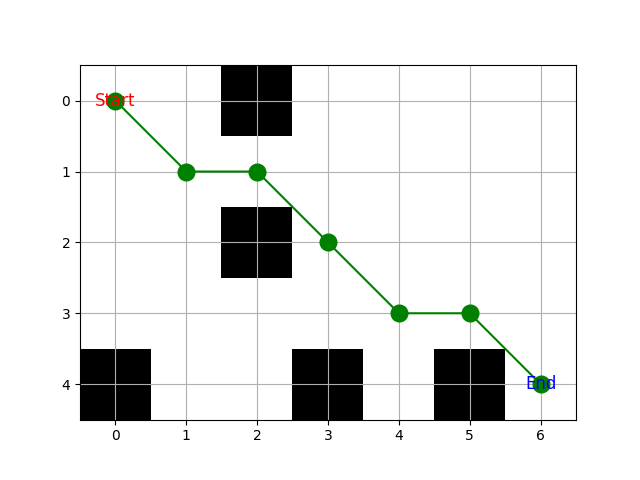
\includegraphics[scale=0.6]{figs/astar4} % Escala la imagen al 150% de su tamaño original
  \caption{ Ejemplo de búsqueda hacia un objetivo con A*.}
  \label{fig:mel}
\end{figure}

